\chapter{The Two Partners}
\label{ch:partners}

The search engine operates as a partnership between two distinct components: the \textbf{Manager} (\texttt{lc0.exe}), which maintains tree bookkeeping and decision selection, and the \textbf{Artist} (the BT3 neural network), which evaluates positions in single forward passes.

\section{The Handshake}

\begin{established}[The Engine-Network Handshake]
The interaction between manager and neural network proceeds step-by-step:
\begin{center}
\begin{minipage}{\linewidth}
\captionsetup{type=figure}
\centering
\subcaptionbox{Manager holds board}{\input{figures/fig_1_1a.tex}}\qquad
\subcaptionbox{Board slides to Artist}{% GENERATED by tools/make_figures.py — do not edit.
\begin{tikzpicture}
  \node[draw=NavyBlue, fill=PaleGrey, rounded corners=3pt, minimum width=24mm, minimum height=14mm, font=\small\bfseries, align=center] (mgr) at (0,0) {MANAGER\\ \scriptsize (lc0.exe)};
  \vgboardnode{board}{(3.4,0)}{4k3/8/4K3/4P3/8/8/8/8 w - - 0 1}{10pt}
  \node[draw=NavyBlue, fill=BuildBlue!15, rounded corners=3pt, minimum width=24mm, minimum height=14mm, font=\small\bfseries, align=center] (art) at (6.8,0) {ARTIST\\ \scriptsize (BT3 Network)};
  \draw[vgpath] (board.east) -- (art.west);
\end{tikzpicture}
}\\[2ex]
\subcaptionbox{Artist returns cards}{% GENERATED by tools/make_figures.py — do not edit.
\begin{tikzpicture}
  \node[draw=NavyBlue, fill=PaleGrey, rounded corners=3pt, minimum width=24mm, minimum height=14mm, font=\small\bfseries, align=center] (mgr) at (0,0) {MANAGER\\ \scriptsize (lc0.exe)};
  \vgboardnode{board}{(3.4,0)}{4k3/8/4K3/4P3/8/8/8/8 w - - 0 1}{10pt}
  \node[draw=NavyBlue, fill=BuildBlue!15, rounded corners=3pt, minimum width=24mm, minimum height=14mm, font=\small\bfseries, align=center] (art) at (6.8,0) {ARTIST\\ \scriptsize (BT3 Network)};
  \draw[vgpath] (board.east) -- (art.west);
  \node[draw=NavyBlue, fill=white, rounded corners=2pt, font=\scriptsize\bfseries, align=center, inner sep=3pt] (pcard) at (3.4, 1.9) {Policy Card};
  \node[draw=NavyBlue, fill=white, rounded corners=2pt, font=\scriptsize\bfseries, align=center, inner sep=3pt] (wdlcard) at (3.4, -1.9) {WDL Card};
  \draw[vgbackprop] (art.north) to[bend right=20] (pcard.east);
  \draw[vgbackprop] (pcard.west) to[bend right=20] (mgr.north);
  \draw[vgbackprop] (art.south) to[bend left=20] (wdlcard.east);
  \draw[vgbackprop] (wdlcard.west) to[bend left=20] (mgr.south);
\end{tikzpicture}
}\qquad
\subcaptionbox{Manager writes node}{\input{figures/fig_1_1d.tex}}
\captionof{figure}{\textbf{FIG-1.1: The handshake cycle.} Manager passes board position to network; network returns policy prior probabilities and single-look WDL value evaluation (Equations~\eqref{eq:E1}--\eqref{eq:E2}).}
\label{fig:1_1}
\end{minipage}
\end{center}
\end{established}

\section{The Problem the Search Has to Solve}
\label{sec:1_2}


\begin{established}[Three Essential Search Constraints]
Before deriving any formula, we set the three requirements (R1--R3) that any MCTS selection rule must satisfy simultaneously:
\begin{center}
% GENERATED by tools/make_figures.py — do not edit.
\begin{tikzpicture}
  \node[draw=NavyBlue, fill=NavyBlue!5, rounded corners=3pt, inner sep=6pt, text width=140mm, font=\small] (title) at (0, 3.6) {
    \textbf{Three Essential Constraints on Search Selection (R1--R3)}\\
    \scriptsize The selection rule must satisfy three competing requirements simultaneously:
  };

  \node[draw=NavyBlue, fill=white, rounded corners=3pt, inner sep=5pt, text width=43mm, font=\scriptsize, align=left] (r1) at (-4.8, 1.4) {
    \textbf{R1: Zero Visits Allowed}\\[0.5ex]
    Most moves must be allowed 0 visits. A 46-move position on a small budget cannot afford 1 visit each.\\[0.5ex]
    \textcolor{PitfallRed}{\textbf{Prevents}: Exhaustive probing.}
  };

  \node[draw=NavyBlue, fill=white, rounded corners=3pt, inner sep=5pt, text width=43mm, font=\scriptsize, align=left] (r2) at (0, 1.4) {
    \textbf{R2: Reachable Later}\\[0.5ex]
    Every legal move must remain reachable later. No move may be permanently excluded.\\[0.5ex]
    \textcolor{PitfallRed}{\textbf{Prevents}: Blind spots.}
  };

  \node[draw=NavyBlue, fill=white, rounded corners=3pt, inner sep=5pt, text width=43mm, font=\scriptsize, align=left] (r3) at (4.8, 1.4) {
    \textbf{R3: Overrule Prior}\\[0.5ex]
    With enough visits, measurement must be able to overrule any prior estimate.\\[0.5ex]
    \textcolor{PitfallRed}{\textbf{Prevents}: Prior stubbornness.}
  };

  \node[draw=IdeaGreen, fill=IdeaGreen!8, line width=0.8pt, rounded corners=3pt, inner sep=6pt, text width=140mm, font=\scriptsize, align=left] (witness) at (0, -1.2) {
    \textbf{Witness Position: Morphy--Brunswick/Isouard (Paris 1858, 15\dots Nxd7)}\\[0.4ex]
    $\bullet$ 46 legal moves. Network prior gives \textbf{Qb8+} only $P = \mathbf{1.60\%}$ (ranked 7th, behind Qb7 31.93\%, Qb5 9.57\%, Qc3 8.33\%).\\[0.4ex]
    $\bullet$ Yet Stockfish (d30) proves \textbf{Qb8+} is a forced mate in 2. Any rule that permanently filters low-prior moves fails here. (\texttt{ch06\_building\_puct.tex:L55})
  };
\end{tikzpicture}

\captionof{figure}{\textbf{FIG-1.7: The problem the search has to solve.} Citing \texttt{ch06\_building\_puct.tex:L55--L64}. Requirements R1 (zero visits allowed), R2 (reachable later), and R3 (overrule prior) pull against each other. Witness: Morphy position after 15\dots Nxd7, where forced mate in 2 (\textbf{Qb8+}) gets only 1.60\% prior attention.}
\label{fig:1_7}
\end{center}
\end{established}

\section{Building the Selection Rule: Attempts 1--3}

\begin{established}[Deriving PUCT: Attempts 1--3]
We test candidate selection rules against requirements R1--R3:
\begin{center}
\begin{minipage}{\linewidth}
\captionsetup{type=figure}
\centering
\subcaptionbox{1. Filter top $k$}[44mm]{% GENERATED by tools/make_figures.py — do not edit.
\begin{tikzpicture}
  \node[draw=NavyBlue, fill=white, rounded corners=3pt, inner sep=4pt, text width=40mm, font=\scriptsize, align=center] (cand) at (0, 1.6) {
    \textbf{Attempt 1}: Search top $k=3$ priors
  };
  \node[draw=PitfallRed, fill=PitfallRed!8, rounded corners=2pt, inner sep=4pt, text width=40mm, font=\scriptsize, align=center] (diag) at (0, 0.1) {
    \textbf{Morphy Top 3}: Qb7 ($31.93\%$), Qb5 ($9.57\%$), Qc3 ($8.33\%$)\\[0.4ex]
    \textcolor{WorkGrey}{\textbf{Qb8+} ($1.60\%$, Mate in 2) is \textbf{EXCLUDED} (0 visits forever)}
  };
  \node[draw=PitfallRed, fill=PitfallRed, text=white, rounded corners=2pt, font=\tiny\bfseries, inner sep=2pt, text width=38mm, align=center] at (0, -1.2) {VIOLATES R2: Blind Spot};
\end{tikzpicture}
}\hfill
\subcaptionbox{2. Add prior}[44mm]{% GENERATED by tools/make_figures.py — do not edit.
\begin{tikzpicture}
  \node[draw=NavyBlue, fill=white, rounded corners=3pt, inner sep=4pt, text width=40mm, font=\scriptsize, align=center] (cand) at (0, 1.6) {
    \textbf{Attempt 2}: Add prior $Q + c \cdot P$ ($c=1$)
  };
  \begin{scope}[shift={(0, -0.1)}]
    \draw[NavyBlue!40, fill=BuildBlue!40] (-1.3, -0.6) rectangle (-0.3, 0.3);
    \draw[NavyBlue!40, fill=GoldPath!40] (-1.3, 0.3) rectangle (-0.3, 0.7);
    \node[font=\scriptsize] at (-0.8, -0.15) {$Q$};
    \node[font=\scriptsize] at (-0.8, 0.5) {$cP$};
    \node[font=\scriptsize\bfseries] at (-0.8, -0.85) {Qb7};

    \draw[NavyBlue!40, fill=BuildBlue!40] (0.3, -0.6) rectangle (1.3, 0.4);
    \draw[NavyBlue!40, fill=GoldPath!40] (0.3, 0.4) rectangle (1.3, 0.5);
    \node[font=\scriptsize] at (0.8, -0.1) {$Q$};
    \node[font=\scriptsize] at (0.8, 0.45) {$cP$};
    \node[font=\scriptsize\bfseries] at (0.8, -0.85) {Qb8+};
  \end{scope}
  \node[draw=PitfallRed, fill=PitfallRed, text=white, rounded corners=2pt, font=\tiny\bfseries, inner sep=2pt, text width=38mm, align=center] at (0, -1.4) {VIOLATES R3: Prior Constant};
\end{tikzpicture}
}\hfill
\subcaptionbox{3. Prior $\cdot$ UCB1}[44mm]{% GENERATED by tools/make_figures.py — do not edit.
\begin{tikzpicture}
  \node[draw=NavyBlue, fill=white, rounded corners=3pt, inner sep=4pt, text width=40mm, font=\scriptsize, align=center] (cand) at (0, 1.6) {
    \textbf{Attempt 3}: $Q + c \cdot P \sqrt{\frac{\ln N}{n}}$
  };
  \begin{scope}[shift={(0, -0.1)}]
    \draw[NavyBlue!40, fill=BuildBlue!40] (-0.8, -0.6) rectangle (-0.2, 0.0);
    \draw[PitfallRed, fill=PitfallRed!30, ->, line width=1.2pt] (-0.5, 0.0) -- (-0.5, 0.8);
    \node[font=\scriptsize\bfseries, text=PitfallRed] at (-0.5, 1.0) {$\infty$ at $n=0$};
    \node[font=\scriptsize\bfseries] at (-0.5, -0.85) {Unvisited};
  \end{scope}
  \node[draw=PitfallRed, fill=PitfallRed, text=white, rounded corners=2pt, font=\tiny\bfseries, inner sep=2pt, text width=38mm, align=center] at (0, -1.4) {VIOLATES R1: Forced 1st Visit};
\end{tikzpicture}
}
\captionof{figure}{\textbf{FIG-1.8: Selection rule attempts 1--3.} Citing \texttt{ch06\_building\_puct.tex:L66--115}. (a) Attempt 1 (top-$k$ filter) fails R2. (b) Attempt 2 ($Q+cP$) fails R3 (prior never decays). (c) Attempt 3 (prior $\cdot$ UCB1) fails R1 ($\infty$ at $n=0$, modifying Equation~\eqref{eq:E7}).}
\label{fig:1_8_part1}
\end{minipage}
\end{center}
\end{established}

\section{The Surviving Rule: Attempts 4--5 \& Final Formula}

Fixing unvisited infinity leads to $\sqrt{N}$ growth and yields the **Predictor + Upper Confidence Bound applied to Trees (PUCT)** selection formula:

\begin{equation}
\label{eq:E10}
\boxed{\;a^* \;=\; \argmax_{a} \left[\; Q(s,a) \;+\; c_{\text{puct}}(N) \cdot P(a \mid s) \cdot \frac{\sqrt{N(s)}}{1 + n_a} \;\right]\;}
\end{equation}

\begin{established}[Deriving PUCT: Attempts 4--5 and Final Form]
\begin{center}
\begin{minipage}{\linewidth}
\captionsetup{type=figure}
\centering
\subcaptionbox{4. Finite at zero}{% GENERATED by tools/make_figures.py — do not edit.
\begin{tikzpicture}
  \node[draw=NavyBlue, fill=white, rounded corners=3pt, inner sep=4pt, text width=65mm, font=\scriptsize, align=center] (cand) at (0, 1.6) {
    \textbf{Attempt 4}: $Q + c \cdot P \frac{\sqrt{\ln N}}{1+n}$
  };
  \node[draw=PitfallRed, fill=PitfallRed!8, rounded corners=2pt, inner sep=4pt, text width=65mm, font=\scriptsize, align=center] (diag) at (0, 0.1) {
    $N = 100 \to 10{,}000$ ($100\times$ search budget):\\[0.4ex]
    $\sqrt{\ln N}$ grows by only \textbf{41\%} ($\sqrt{2} = 1.41$)\\[0.4ex]
    Neglected move needs \textbf{10$\times$} growth to overcome prior deficit
  };
  \node[fill=PitfallRed, text=white, rounded corners=2pt, font=\scriptsize\bfseries, inner sep=3pt] at (0, -1.2) {VIOLATES R2: Neglected Move Frozen};
\end{tikzpicture}
}\qquad
\subcaptionbox{5. $\sqrt{N}$ growth}{% GENERATED by tools/make_figures.py — do not edit.
\begin{tikzpicture}
  \node[draw=IdeaGreen, fill=IdeaGreen!8, rounded corners=3pt, inner sep=4pt, text width=65mm, font=\scriptsize, align=center] (cand) at (0, 1.6) {
    \textbf{Attempt 5}: $Q + c_{\mathrm{puct}} \cdot P \frac{\sqrt{N}}{1+n}$
  };
  \node[draw=IdeaGreen, fill=white, rounded corners=2pt, inner sep=4pt, text width=65mm, font=\scriptsize, align=center] (diag) at (0, 0.1) {
    $N = 100 \to 10{,}000$ ($100\times$ search budget):\\[0.4ex]
    $\sqrt{N}$ grows \textbf{10-fold} ($10 \to 100$)\\[0.4ex]
    Neglected move gets its turn!
  };
  \node[fill=IdeaGreen, text=white, rounded corners=2pt, font=\scriptsize\bfseries, inner sep=3pt] at (0, -1.2) {SURVIVOR: Satisfies R1, R2, R3};
\end{tikzpicture}
}\\[2ex]
% GENERATED by tools/make_figures.py — do not edit.

\begin{tikzpicture}
  \node[draw=NavyBlue, fill=NavyBlue!5, rounded corners=4pt, inner sep=8pt, font=\small, text width=140mm, align=center] (formula) {
    $\mathbf{E10:\ a^* = \argmax_a \left[\; \underbrace{Q(s,a)}_{\text{what I measured}} + \underbrace{c_{\mathrm{puct}} \cdot P(a \mid s) \cdot \frac{\sqrt{N(s)}}{1+N(s,a)}}_{U(s,a):\ \text{what I haven't checked}} \;\right]}$
  };
\end{tikzpicture}

\captionof{figure}{\textbf{FIG-1.9: Selection rule attempts 4--5 and final formula.} Citing \texttt{ch06\_building\_puct.tex:L116--149}. (a) Attempt 4 ($\sqrt{\ln N}$ growth) fails R2 in practice because neglected moves stay frozen. (b) Attempt 5 ($\sqrt{N}$ growth) survives R1--R3. Boxed: The complete PUCT selection formula (Equation~\eqref{eq:E10}).}
\label{fig:1_8_part2}
\end{minipage}
\end{center}
\end{established}

\section{Reading the Finished Formula, Term by Term}

Total score $S(a) = Q(a) + U(a)$ combines exploitation $Q(a)$ and exploration $U(a)$. Unvisited nodes inherit an unvisited baseline floor $Q_{\text{FPU}}$:

\begin{equation}
\label{eq:E11}
\boxed{\;Q_{\text{FPU}} \;=\; Q(\text{parent}) \;-\; c_{\text{fpu}}\sqrt{\sum_{\text{visited}} P}\;}
\end{equation}

while the CPUCT exploration scaling parameter grows logarithmically with node visit count $N$:

\begin{equation}
\label{eq:E12}
\boxed{\;c_{\text{puct}}(N) \;=\; c_{\text{base}} \;+\; c_{\text{factor}}\,\ln\left(\frac{N + c_{\text{mod}}}{c_{\text{mod}}}\right)\;}
\end{equation}

\begin{established}[Math Formula Overview]
\begin{center}
\input{figures/fig_1_10.tex}
\captionof{figure}{\textbf{FIG-1.10: Math formula overview diagram.} Total score $S(a) = Q(a) + U(a)$ defined by Equation~\eqref{eq:E10}. Exploitation $Q(a)$ (solid bar) uses Equation~\eqref{eq:E4} for visited moves and $Q_{\text{FPU}}$ (Equation~\eqref{eq:E11}) for unvisited moves. Exploration $U(a)$ scales with $c_{\text{puct}}(N)$ (Equation~\eqref{eq:E12}). Visiting a move increments $(1+n_a)$, shrinking $U(a)$ (see FIG-2.2).}
\label{fig:1_10}
\end{center}
\end{established}

\section{Term-by-Term Reasoning}

\begin{established}[Term-by-Term Reasoning]
The four core design questions behind the formula's terms:
\begin{center}
\begin{minipage}{\linewidth}
\captionsetup{type=figure}
\centering
\subcaptionbox{Why $Q$ is an average}{% GENERATED by tools/make_figures.py — do not edit.
\begin{tikzpicture}
  \node[draw=BuildBlue, fill=BuildBlue!8, rounded corners=3pt, inner sep=5pt, text width=66mm, font=\scriptsize, align=left] (box) {
    \textbf{(a) Why $Q$ is an average \& starts as a guess}\\[0.6ex]
    • $Q(s,a)$ is running mean of leaf evaluations (E4).\\[0.4ex]
    • Unvisited moves start at $Q_{\mathrm{FPU}} = Q(\mathrm{root}) - 0.33\sqrt{\sum P_{\mathrm{vis}}}$ (E11).\\[0.4ex]
    • \textcolor{PitfallRed}{$Q=0$ fails}: slander in win, optimism in loss.\\[0.4ex]
    • \textcolor{PitfallRed}{$Q=Q(\mathrm{parent})$ fails}: unvisited ties with measured. (See FIG-2.B)
  };
\end{tikzpicture}
}\qquad
\subcaptionbox{Why $U$ is built this way}{% GENERATED by tools/make_figures.py — do not edit.
\begin{tikzpicture}
  \node[draw=GoldPath, fill=GoldPath!10, rounded corners=3pt, inner sep=5pt, text width=66mm, font=\scriptsize, align=left] (box) {
    \textbf{(b) Why $U$ is built the way it is}\\[0.6ex]
    • $P$ in numerator: Move with low prior gets small initial claim.\\[0.4ex]
    • $\sqrt{N}$ in numerator: Claim of neglected move \textbf{grows} as search spends elsewhere (forces visit in FIG-3.1, finds Qb8+ in FIG-4.1).\\[0.4ex]
    • $(1+n_a)$ in denominator: Visiting a move \textbf{halves} its claim immediately (halving decides pick in FIG-2.2).
  };
\end{tikzpicture}
}\\[2ex]
\subcaptionbox{Why $S=Q+U$ is a sum}{% GENERATED by tools/make_figures.py — do not edit.
\begin{tikzpicture}
  \node[draw=NavyBlue, fill=PaleGrey, rounded corners=3pt, inner sep=5pt, text width=66mm, font=\scriptsize, align=left] (box) {
    \textbf{(c) Why $S = Q + U$ is a sum \& Priority Nature}\\[0.6ex]
    • $Q$ = how good it looked; $U$ = how much still unknown. Neither can veto the other.\\[0.4ex]
    • $S$ is a \textbf{priority score} (where to look next), NOT an evaluation or probability.\\[0.4ex]
    • \textbf{The Trap}: Leading $S$ falls from $1.764 \to 1.400$ across FIG-2.0$\to$2.8. $Q$ stays flat ($+0.976 \to +0.968$); fall is 100\% $U$ decay!
  };
\end{tikzpicture}
}\qquad
\subcaptionbox{Why $c_{\mathrm{puct}}$ grows}{% GENERATED by tools/make_figures.py — do not edit.
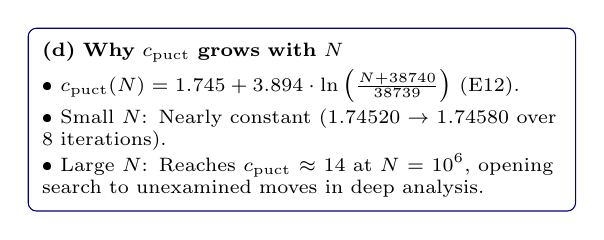
\begin{tikzpicture}
  \node[draw=NavyBlue, fill=white, rounded corners=3pt, inner sep=5pt, text width=66mm, font=\scriptsize, align=left] (box) {
    \textbf{(d) Why $c_{\mathrm{puct}}$ grows with $N$}\\[0.6ex]
    • $c_{\mathrm{puct}}(N) = 1.745 + 3.894\cdot \ln\left(\frac{N+38740}{38739}\right)$ (E12).\\[0.4ex]
    • Small $N$: Nearly constant ($1.74520 \to 1.74580$ over 8 iterations).\\[0.4ex]
    • Large $N$: Reaches $c_{\mathrm{puct}} \approx 14$ at $N=10^6$, opening search to unexamined moves in deep analysis.
  };
\end{tikzpicture}
}
\captionof{figure}{\textbf{FIG-1.11: Term-by-term breakdown.} Citing \texttt{ch06\_building\_puct.tex:L150--273}. (a) $Q$ is evidence (Equation~\eqref{eq:E4}); unvisited moves inherit penalized $Q_{\text{FPU}}$ floor (Equation~\eqref{eq:E11}). (b) $P$, $\sqrt{N}$, and $(1+n_a)$ in Equation~\eqref{eq:E10} balance initial claim, search growth, and immediate decay. (c) $S$ is a priority score, not an evaluation; falling $S$ is 100\% $U$ decay. (d) $c_{\text{puct}}(N)$ (Equation~\eqref{eq:E12}) opens search during deep analysis.}
\label{fig:1_11}
\end{minipage}
\end{center}
\end{established}

\section{Anatomy of a Tree Node}

A search tree node stores these specific fields \textbf{because} the selection rule derived in §1.4 (Equation~\eqref{eq:E10}) needs them to evaluate candidate moves.

\begin{established}[Search Tree Node Anatomy]
Each node in the MCTS search tree stores both measured network feedback and running statistics:
\begin{center}
% GENERATED by tools/make_figures.py — do not edit.
\begin{tikzpicture}
  \node[vgroot, minimum width=45mm, minimum height=22mm, inner sep=6pt] (node) at (0,0) {
    \textbf{Kd6}\\[0.5ex]
    $P(a) = 45.13\% \quad n_a = 4$\\[0.3ex]
    $Q(a) = \mathbf{+0.98394} \quad V = \mathbf{+0.97602}$\\[0.3ex]
    $U(a) = 0.41691 \quad S(a) = 1.40085$
  };
  \node[right=8mm of node, font=\scriptsize, text width=55mm, align=left] (callouts) {
    $\bullet$ \textbf{Move}: Kd6 candidate move\\
    $\bullet$ \textbf{P}: Prior policy probability from network\\
    $\bullet$ \textbf{n}: Visit count spent on this branch\\
    $\bullet$ \textbf{Q}: Running average evaluation\\
    $\bullet$ \textbf{V}: Node's own single-look evaluation\\
    $\bullet$ \textbf{U}: Curiosity / exploration bonus\\
    $\bullet$ \textbf{S}: Total score $S = Q + U$ (decides pick)
  };
\end{tikzpicture}

\captionof{figure}{\textbf{FIG-1.2: Node Anatomy.} Prior probability $P(a)$, visit count $n_a$, running average evaluation $Q(a)$ (Equation~\eqref{eq:E4}), single-pass value $V$ (Equation~\eqref{eq:E2}), curiosity bonus $U(a)$, and selection score $S(a) = Q(a) + U(a)$ (Equation~\eqref{eq:E10}).}
\label{fig:1_2}
\end{center}
\end{established}

\section{The Initial Network Evaluation}

\begin{realdata}[Initial Position Assessment]
For our subject endgame position (\texttt{4k3/8/4K3/4P3/8/8/8/8 w - - 0 1}), one single forward pass produces initial policy priors and win-draw-loss assessment:
\begin{center}
\begin{minipage}{\linewidth}
\captionsetup{type=figure}
\centering
\subcaptionbox{Cards Face-Down}{% GENERATED by tools/make_figures.py — do not edit.
\begin{tikzpicture}
  \vgboardnode{board}{(0,0)}{4k3/8/4K3/4P3/8/8/8/8 w - - 0 1}{10pt}
  \node[draw=NavyBlue, fill=PaleGrey, rounded corners=3pt, inner sep=5pt, right=6mm of board, text width=48mm, font=\scriptsize] (card1) {
    \textbf{Policy Card (Prior Attention)}\\[0.5ex]
    Kd6: \textbf{45.13\%} \quad Kf6: \textbf{44.23\%}\\[0.3ex]
    Kf5: 5.38\% \quad Kd5: 5.26\%
  };
  \node[draw=NavyBlue, fill=white, rounded corners=3pt, inner sep=5pt, below=3mm of card1, text width=48mm, font=\scriptsize] (card2) {
    \textbf{WDL Card (Face Down)}\\[0.5ex]
    \textit{Evaluating position...}
  };
\end{tikzpicture}
}\qquad
\subcaptionbox{Evaluated Numbers}{% GENERATED by tools/make_figures.py — do not edit.
\begin{tikzpicture}
  \vgboardnode{board}{(0,0)}{4k3/8/4K3/4P3/8/8/8/8 w - - 0 1}{10pt}
  \node[draw=NavyBlue, fill=PaleGrey, rounded corners=3pt, inner sep=5pt, right=6mm of board, text width=48mm, font=\scriptsize] (card1) {
    \textbf{Policy Card (Prior Attention)}\\[0.5ex]
    Kd6: \textbf{45.13\%} \quad Kf6: \textbf{44.23\%}\\[0.3ex]
    Kf5: 5.38\% \quad Kd5: 5.26\%
  };
  \node[draw=IdeaGreen, fill=IdeaGreen!8, line width=0.8pt, rounded corners=3pt, inner sep=5pt, below=3mm of card1, text width=48mm, font=\scriptsize] (card2) {
    \textbf{WDL Card (Evaluated)}\\[0.5ex]
    $V = \mathbf{+0.97602}$ \quad $d = \mathbf{0.024}$
  };
\end{tikzpicture}
}
\captionof{figure}{\textbf{FIG-1.3: Policy and WDL cards for K+P endgame.} The policy places 89.36\% of attention on winning moves (Kd6 45.13\%, Kf6 44.23\%), but still leaves 10.64\% on drawing moves (Kf5 5.38\%, Kd5 5.26\%). Initial root value $V = +0.97602$ (Equation~\eqref{eq:E2}), $d = 0.024$.}
\label{fig:1_3}
\end{minipage}
\end{center}

\begin{keyidea}
The network policy is an informed initial instinct, not an unassailable oracle. $89.36\%$ of its attention went to winning moves, but $10.64\%$ remained on moves that throw away the win. The search exists to verify and refine this instinct.
\end{keyidea}
\end{realdata}

\section{One Value Per Position, Not Per Move}

\begin{pitfall}[title={Where People Go Wrong: One Value Per Position, Not Per Move}]
A common misreading assumes the neural network outputs individual value evaluations for candidate moves:
\begin{center}
\begin{minipage}{\linewidth}
\captionsetup{type=figure}
\centering
\subcaptionbox{The Misreading}{% GENERATED by tools/make_figures.py — do not edit.
\begin{tikzpicture}
  \node[draw=NavyBlue, fill=white, rounded corners=3pt, inner sep=5pt, text width=65mm, font=\scriptsize, align=center] (boxa) {
    \textbf{Kd6}: $P{=}45.13\%, V{=}V_1$ \quad \textbf{Kf6}: $P{=}44.23\%, V{=}V_2$\\[0.4ex]
    \textbf{Kf5}: $P{=}5.38\%, V{=}V_3$ \quad \textbf{Kd5}: $P{=}5.26\%, V{=}V_4$
  };
  \draw[PitfallRed, line width=1.8pt] (boxa.north west) -- (boxa.south east);
  \draw[PitfallRed, line width=1.8pt] (boxa.south west) -- (boxa.north east);
  \node[below=2mm of boxa, font=\scriptsize\bfseries, text=PitfallRed, align=center] {The network NEVER outputs a value per move!};
\end{tikzpicture}
}\qquad
\subcaptionbox{What Actually Comes Back}{% GENERATED by tools/make_figures.py — do not edit.
\begin{tikzpicture}
  \node[draw=IdeaGreen, fill=IdeaGreen!8, line width=0.8pt, rounded corners=3pt, inner sep=5pt, text width=65mm, font=\scriptsize, align=center] (boxb) {
    \textbf{One Position Evaluation}: $V(\mathrm{root}) = +0.97602, d = 0.024$\\[0.4ex]
    \textbf{One Policy Distribution}: $P = \{45.13\%, 44.23\%, 5.38\%, 5.26\%\}$
  };
  \node[below=2mm of boxb, font=\scriptsize\itshape, text=WorkGrey, text width=68mm, align=center] {
    One $V$ for the position, four $P$'s for moves. A move gets a value only when expanded into a child position ($V(\mathrm{leaf}) = +0.96766$ in FIG-2.1).
  };
\end{tikzpicture}
}
\captionof{figure}{\textbf{FIG-1.4: One value per position, not one per move.} (a) The network does not produce individual $V$ evaluations for candidate moves. (b) A forward pass returns exactly one $V(s)$ (Equation~\eqref{eq:E2}) for the current position, alongside policy prior probabilities $P(a \mid s)$ for legal moves. A move receives its own value only when expanded into a child position (see FIG-2.1).}
\label{fig:1_4}
\end{minipage}
\end{center}
\end{pitfall}

\vspace{1ex}

\begin{established}[What the Policy Actually Predicts]
The policy prior distribution $P(a \mid s)$ is a fast neural approximation of search preference, not an objective move quality score:
\begin{center}
% GENERATED by tools/make_figures.py — do not edit.
\begin{tikzpicture}
  \node[draw=NavyBlue, fill=PaleGrey, rounded corners=3pt, inner sep=6pt, text width=125mm, font=\small] (claim) at (0,0) {
    \textbf{What the Policy Head Models:}\\[0.5ex]
    \textit{"The policy head predicts \textbf{which move a full search by this same engine would end up preferring}. It is a fast approximation of its own slow self. It is not a model of human choice, not a goodness score, and not calibrated to any rating band."} (\texttt{ch12\_two\_heads.tex:L96})
  };

  \node[draw=PitfallRed, fill=PitfallRed!8, rounded corners=3pt, inner sep=5pt, text width=58mm, font=\scriptsize, below left=4mm and -28mm of claim] (ex1) {
    \textbf{1. Policy is NOT goodness (Downward)}\\[0.3ex]
    Kf5 and Kd5 hold \textbf{10.64\%} of root policy, yet both throw away a won game ($Q=0.000$, SF d30 0.00). (See FIG-4.3)
  };

  \node[draw=IdeaGreen, fill=IdeaGreen!8, rounded corners=3pt, inner sep=5pt, text width=58mm, font=\scriptsize, below right=4mm and -28mm of claim] (ex2) {
    \textbf{2. Policy is NOT goodness (Upward)}\\[0.3ex]
    In Morphy position, $P(\text{Qb8+}) = \mathbf{1.60\%}$ on a forced mate in two. Search overrides policy to find win. (See FIG-5.3)
  };
\end{tikzpicture}

\captionof{figure}{\textbf{FIG-1.5: What the policy predicts.} Citing \texttt{ch12\_two\_heads.tex:L96}. Measured proofs: 10.64\% of root policy goes to losing blunders (FIG-4.3), while a forced mate in 2 receives only 1.60\% prior attention (FIG-5.3).}
\label{fig:1_5}
\end{center}
\end{established}

\section{The Four-Phase Iteration Loop}

\begin{established}[The Four-Phase Loop]
Every single search iteration follows a continuous four-phase loop (Selection $\rightarrow$ Expansion $\rightarrow$ Evaluation $\rightarrow$ Backpropagation):
\begin{center}
\begin{minipage}{\linewidth}
\captionsetup{type=figure}
\centering
\subcaptionbox{1. Selection}{\input{figures/fig_1_6a.tex}}\qquad
\subcaptionbox{2. Expansion}{\input{figures/fig_1_6b.tex}}\\[2ex]
\subcaptionbox{3. Evaluation}{\input{figures/fig_1_6c.tex}}\qquad
\subcaptionbox{4. Backpropagation}{% GENERATED by tools/make_figures.py — do not edit.

\begin{tikzpicture}
  \node[draw=NavyBlue, fill=white, rounded corners=3pt, minimum width=24mm, minimum height=8mm, font=\scriptsize\bfseries] (p1) at (0, 1.2) {1. Selection};
  \node[draw=NavyBlue, fill=white, rounded corners=3pt, minimum width=24mm, minimum height=8mm, font=\scriptsize\bfseries] (p2) at (3.2, 1.2) {2. Expansion};
  \node[draw=NavyBlue, fill=white, rounded corners=3pt, minimum width=24mm, minimum height=8mm, font=\scriptsize\bfseries] (p3) at (3.2, -1.2) {3. Evaluation};
  \node[draw=GoldPath, fill=GoldPath!25, line width=1.2pt, rounded corners=3pt, minimum width=24mm, minimum height=8mm, font=\scriptsize\bfseries] (p4) at (0, -1.2) {4. Backprop};
  \draw[vgedge] (p1) -- (p2);
  \draw[vgedge] (p2) -- (p3);
  \draw[vgedge] (p3) -- (p4);
  \draw[vgedge] (p4) -- (p1);
  \node[draw=NavyBlue, fill=PaleGrey, rounded corners=3pt, inner sep=4pt, below=3mm of p4, anchor=north west, text width=68mm, font=\scriptsize] at (-0.4, -1.6) {\textbf{Backpropagation}: Value $+0.96766$ returns to root, updating $N=1, Q=+0.97184$.};
\end{tikzpicture}
}
\captionof{figure}{\textbf{FIG-1.6: The four-phase MCTS iteration cycle.} Citing \texttt{ch05\_machines\_to\_trees.tex}. Each search iteration executes four sequential steps: Selection (choosing $\max S = Q+U$ via Equation~\eqref{eq:E10}), Expansion (creating child node), Evaluation (single forward pass on leaf), and Backpropagation (updating $N$ and $Q$ via Equation~\eqref{eq:E4} and sign flip Equation~\eqref{eq:E8} along path back to root).}
\label{fig:1_6}
\end{minipage}
\end{center}
\end{established}
